
\section{Modeling in Ptolemy}
\label{sec:modeling-ptolemy}

In this section, we present our work in Ptolemy that models the MAC layer of OpenWSN\footnote{Though the model in each figure is vector graphics, you can zoom in and read the details. We strongly suggest reader to open our Ptolemy model for details. These figures are mainly for illustration purpose.}.

\begin{figure}[t]
\centering
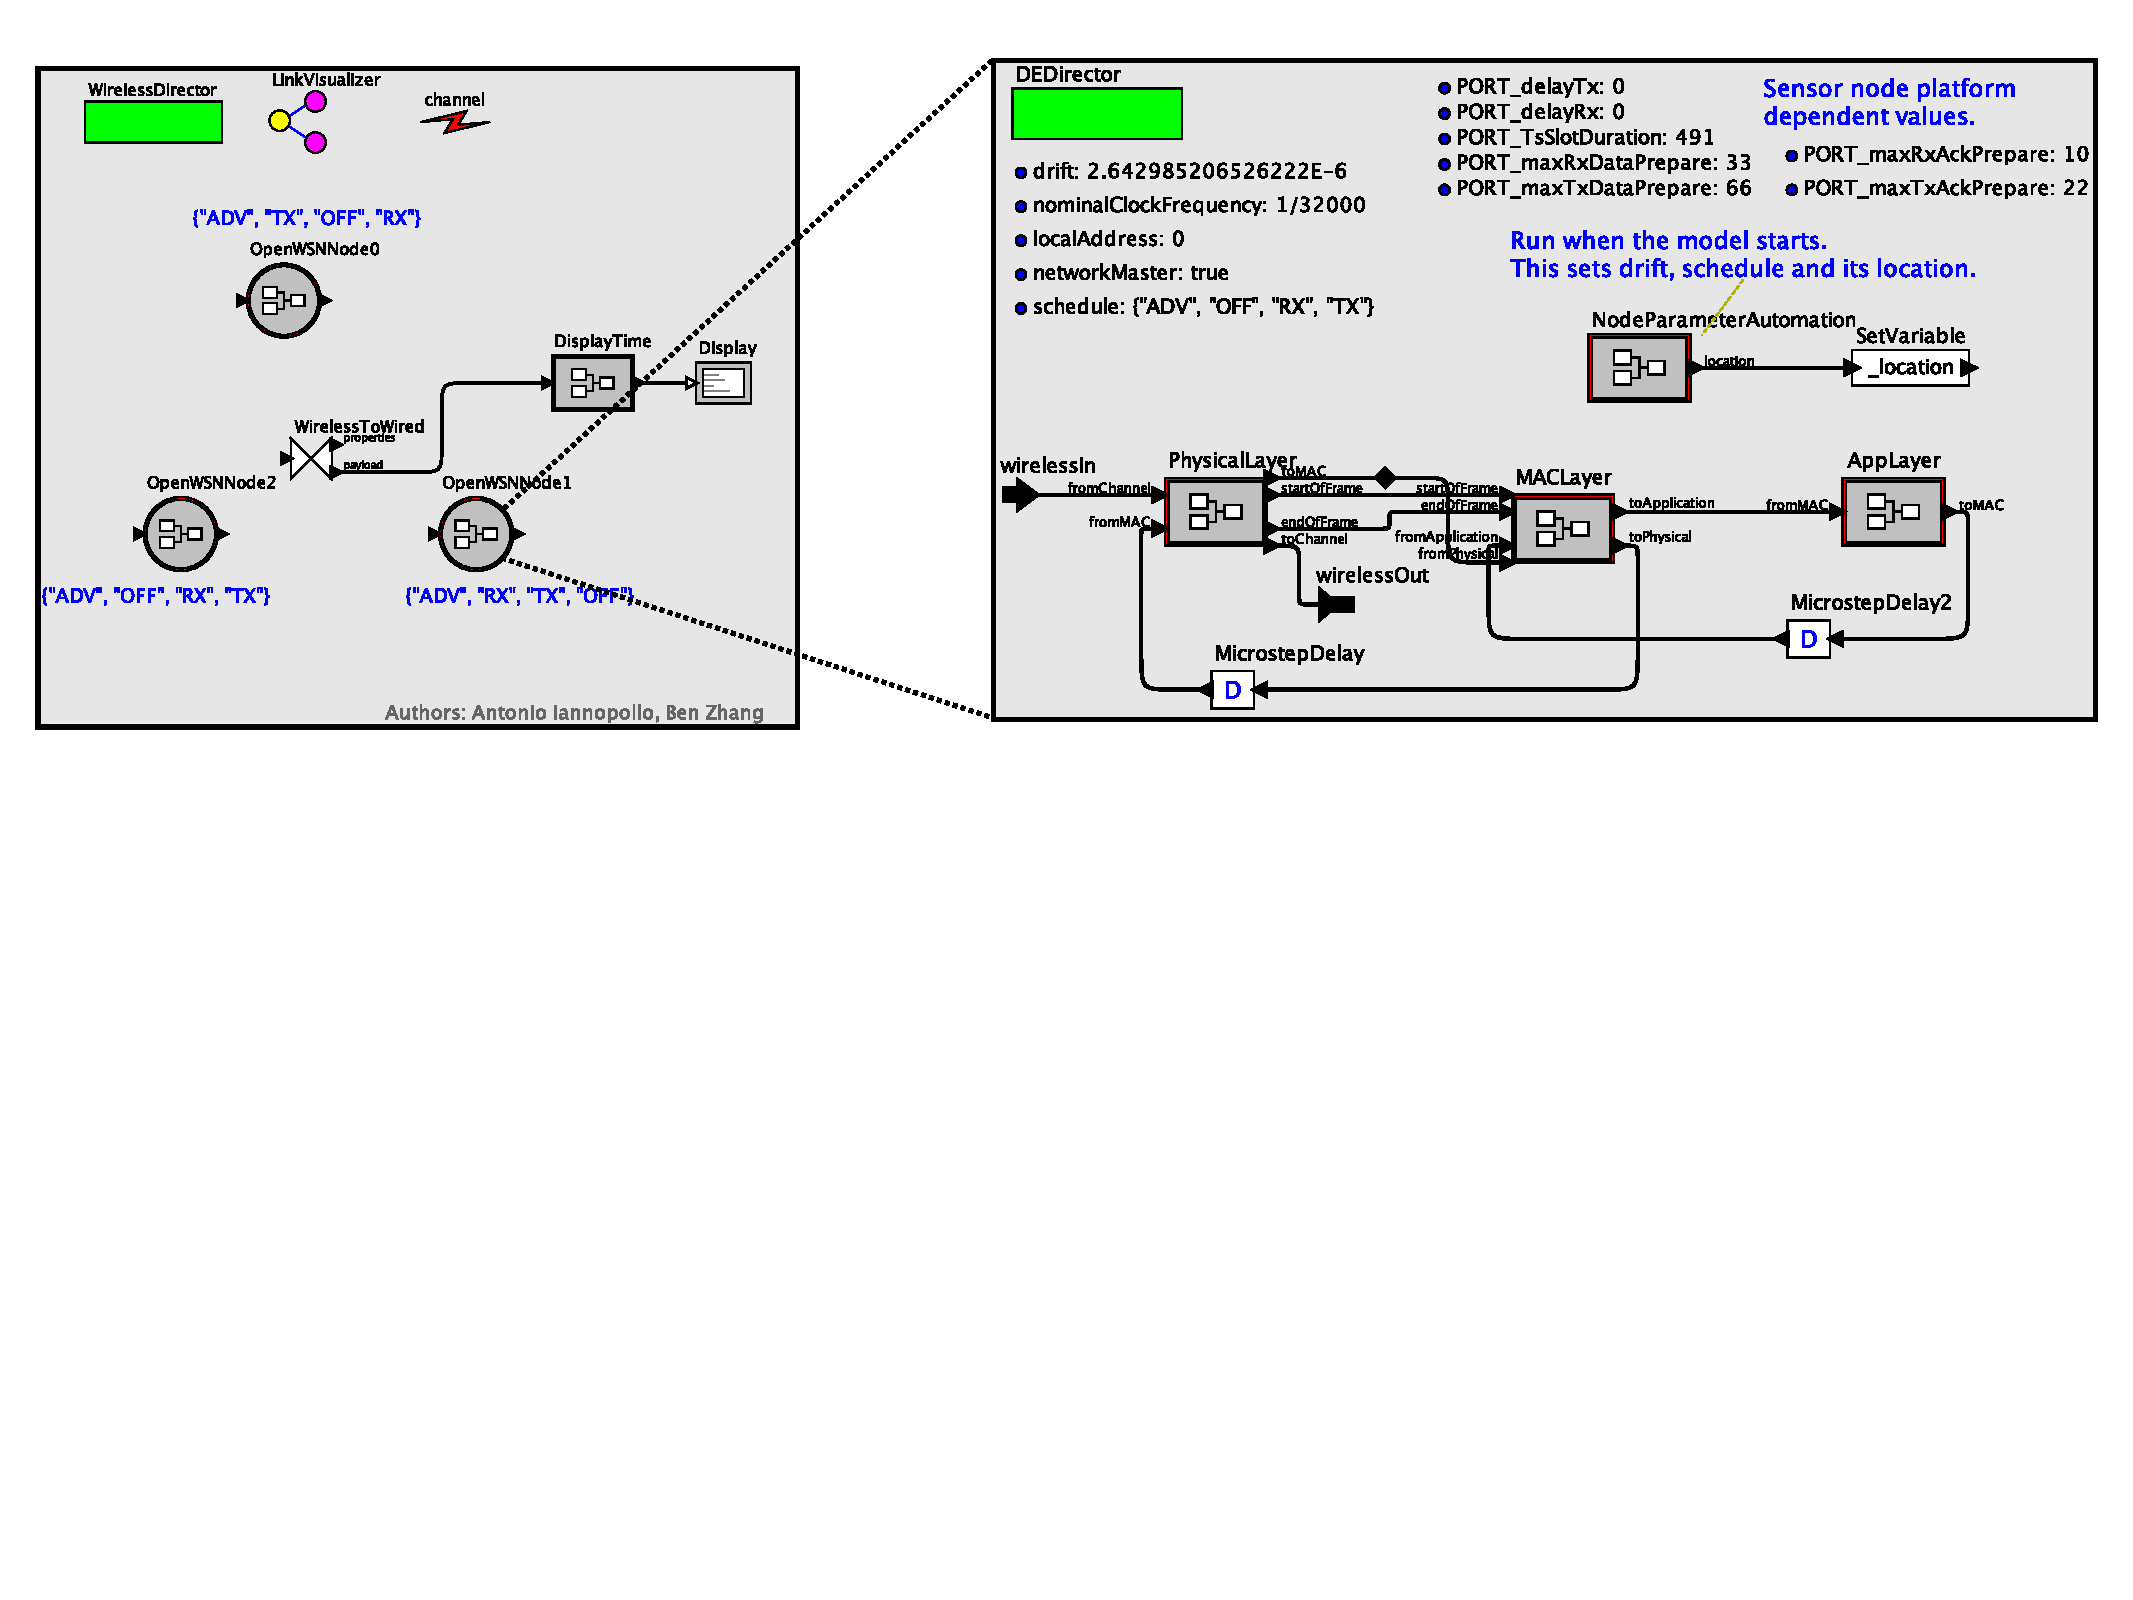
\includegraphics[width=1\columnwidth]{figures/PaperOpenWSNNode}
\caption{An example application of three nodes ({\em left}) and the simplified network stack ({\em right}).}
\label{fig:OpenWSNNode}
\end{figure}

Though our focus is on the TSCH state machine, we have also modeled a simple physical radio and abstracted the higher network layers as a single application layer (see Figure~\ref{fig:OpenWSNNode}). The interface to the Physical layer is mainly achieved with 1) \texttt{startOfFrame} and \texttt{endOfFrame} ports, which indicate the radio status; 2) \texttt{fromPhysical} and \texttt{toPhysical}ports, which convey the payload. The interface to the Application layer is through \texttt{fromMAC} and \texttt{toMAC} ports. 

Inside the \texttt{MACLayer} composite actor, we have a few actors including \texttt{packetQueueManager}, \texttt{scheduler}, \texttt{PacketProcessor} and \texttt{TSCHStateMachine} (names are self explanatory). The most relevant part is the \texttt{TSCHStateMachine}, where we modeled the protocol behavior using Hierarchical Modal Models \ref{fig:TSCHSM}. It consists of five main states, which describe the node activity: \texttt{init}, \texttt{SLEEP}, \texttt{synchronization}, \texttt{tx} and \texttt{rx}. 


\begin{figure}[t]
\centering
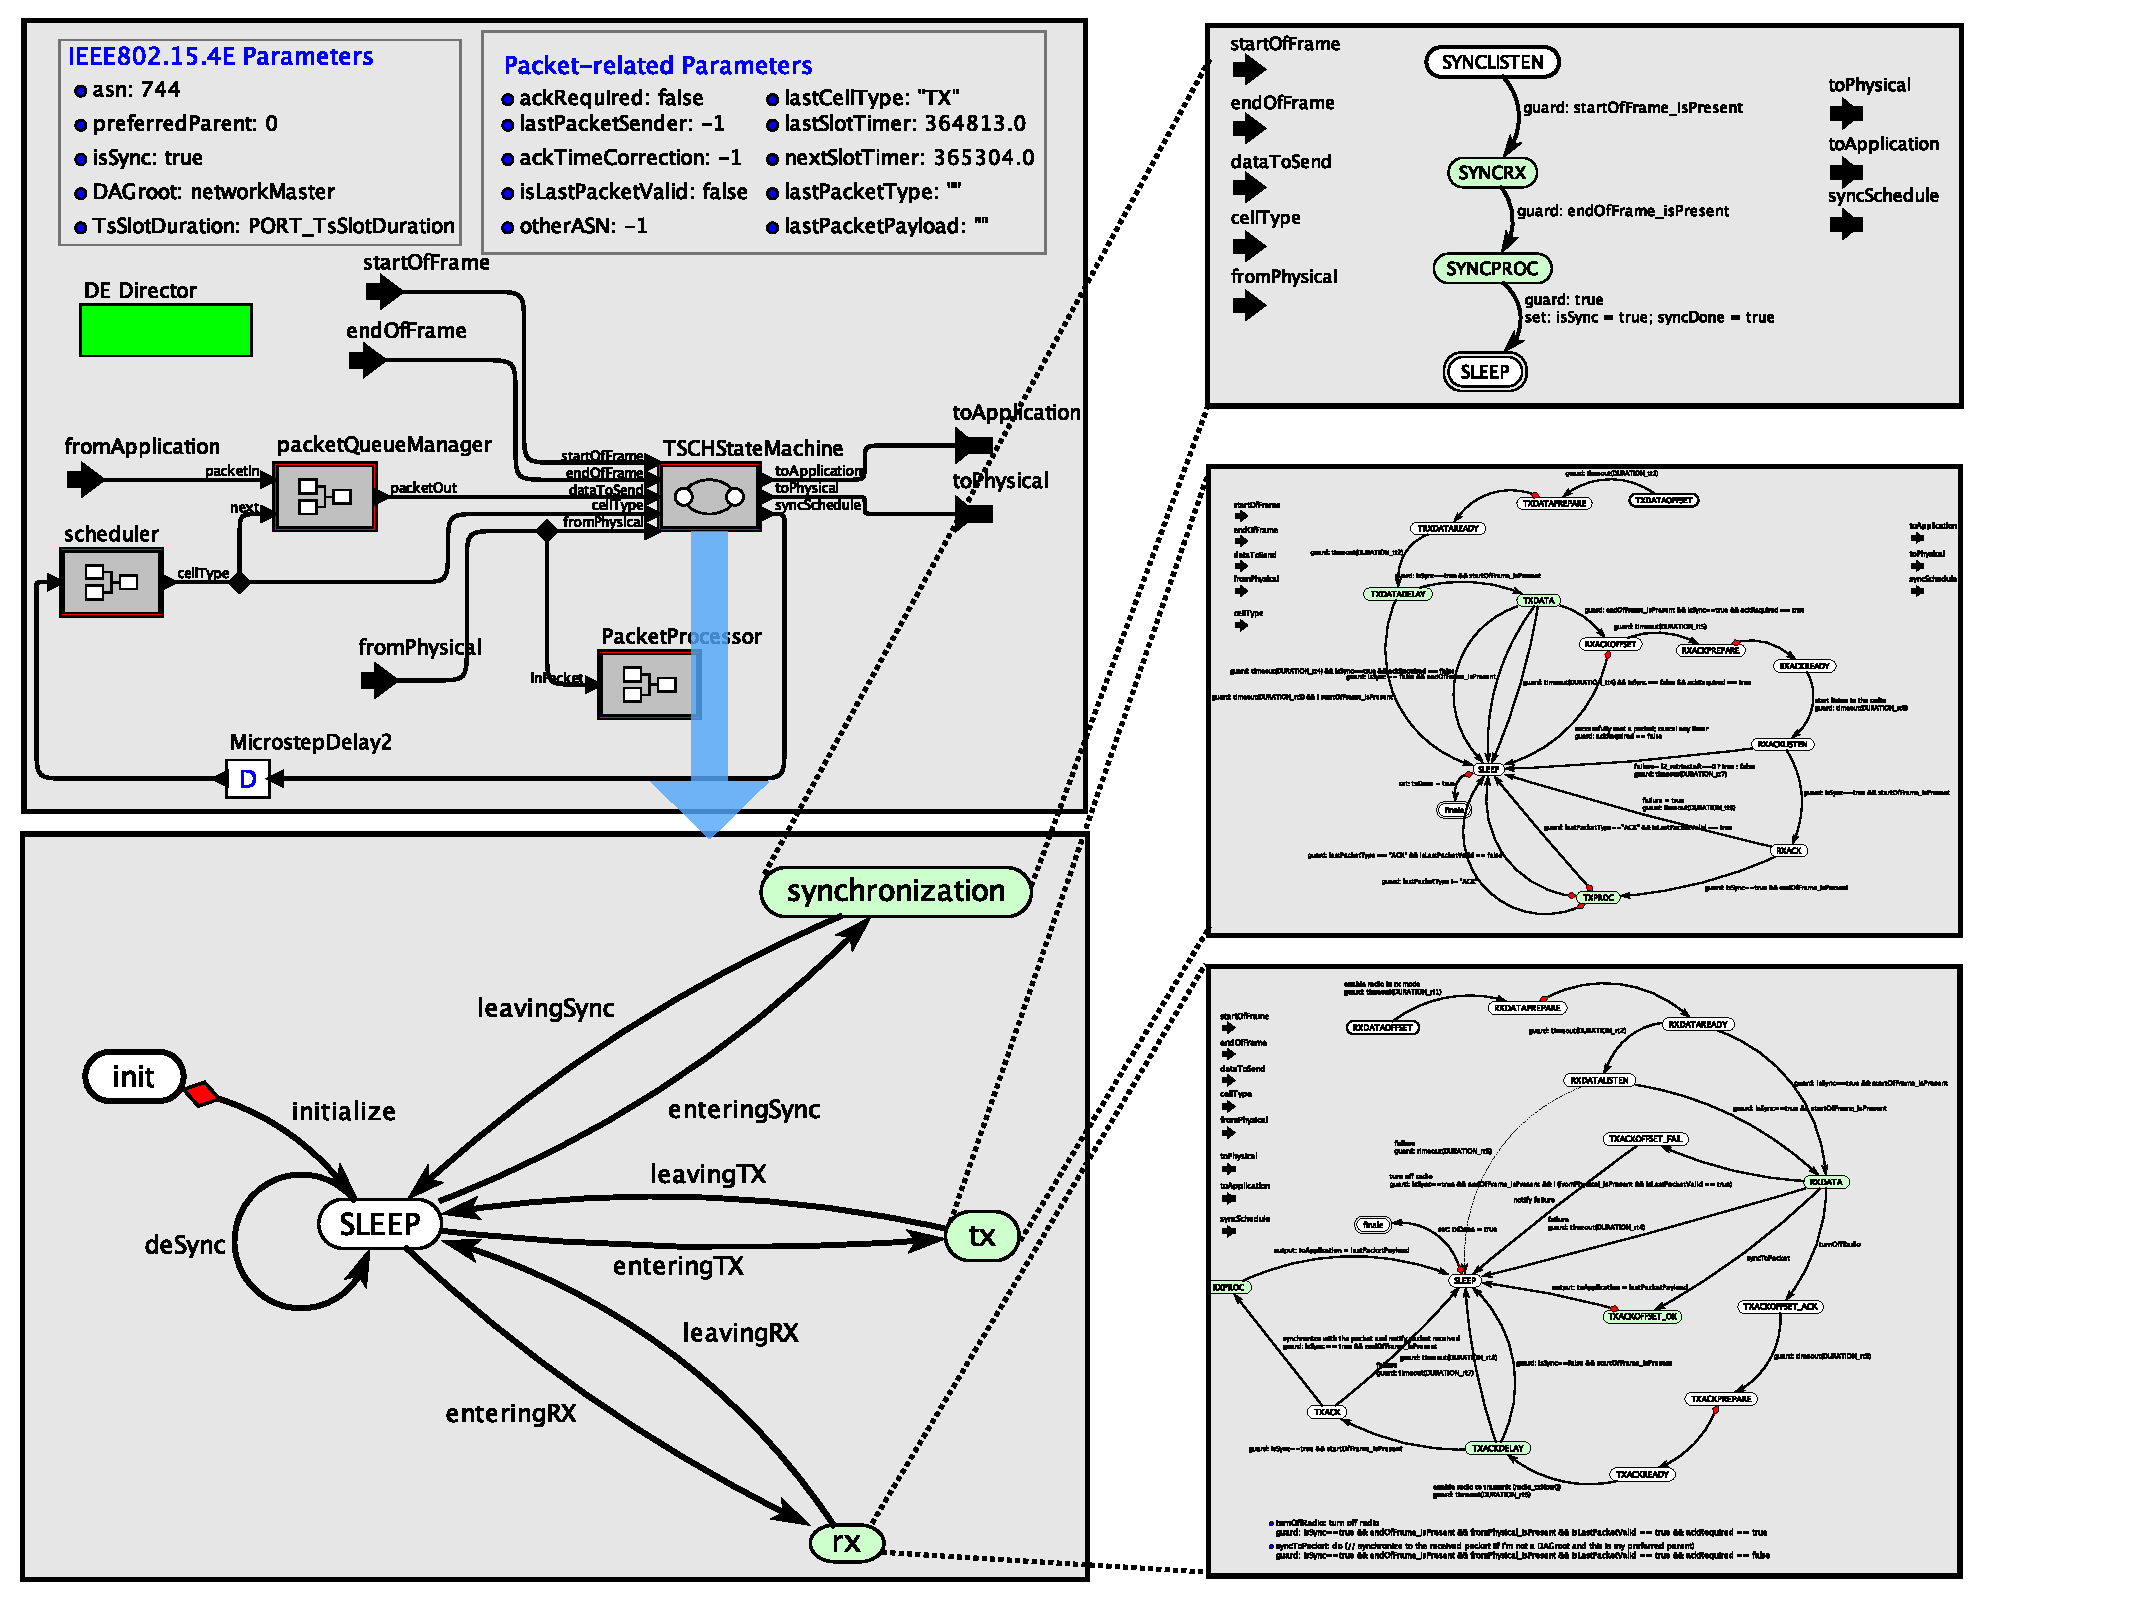
\includegraphics[width=1\columnwidth]{figures/PaperTSCHStateMachine}
\caption{The state machine with refinements of TSCH protocol.}
\label{fig:TSCHSM}
\end{figure}

During the initialization phase, we reset all protocol related parameters, When in the \texttt{synchronization} refinement, the node keeps listening for \texttt{ADV} packet and performs slot synchronization and ASN synchronization. Once the synchronization is done, it goes back to \texttt{SLEEP} state.
The scheduler decides node actions: 
\begin{itemize}
\item If the slot is \texttt{ADV} slot, then the node enters the \texttt{tx} state and sends an \texttt{ADV} packet. 
\item If it's \texttt{TX} or \texttt{RXTX} slot and the node has data to send (there are packets queued at \texttt{packetQueueManager}), it will enter \texttt{tx} state and send the data packet. 
\item If it's \texttt{RX} slot, or it's \texttt{RXTX} slot but the application doesn't have data to send, the node will enter \texttt{rx} state and listen for packets.
\end{itemize}

In \texttt{tx} and \texttt{rx} states, there is a refinement which captures the complicated state transition of the radio. For example, when the node is sending a packet, it first wait a certain time (in \texttt{TXDATAOFFSET} state), then prepares the data for radio to transmit (\texttt{TXDATAPREPARE}), and after a few other states that are used to check the radio status, etc., it finally enters \texttt{TXDATA} state and transmits the packet. Similar complexity exists for managing acknowledgement and receiving a packet. Given our space constraints, we refer the reader to our Ptolemy model for more details on state transition behavior.

The \texttt{synchronization} state is only entered when the node is not synchronized to the rest of the network anymore. Additionally, for every received packet, the node will capture the reception time (Figure~\ref{fig:timeCorrection} {\em up}). If the packet is from a time master, it will calculate the time discrepancy and use it to adjust its synchronization (Figure~\ref{fig:timeCorrection} {\em middle}). If the packet is from a time slave, then the node will still perform a calculation and send the time correction through \texttt{ACK} packet (Figure~\ref{fig:timeCorrection} {\em down}).

\begin{figure}[t]
\centering
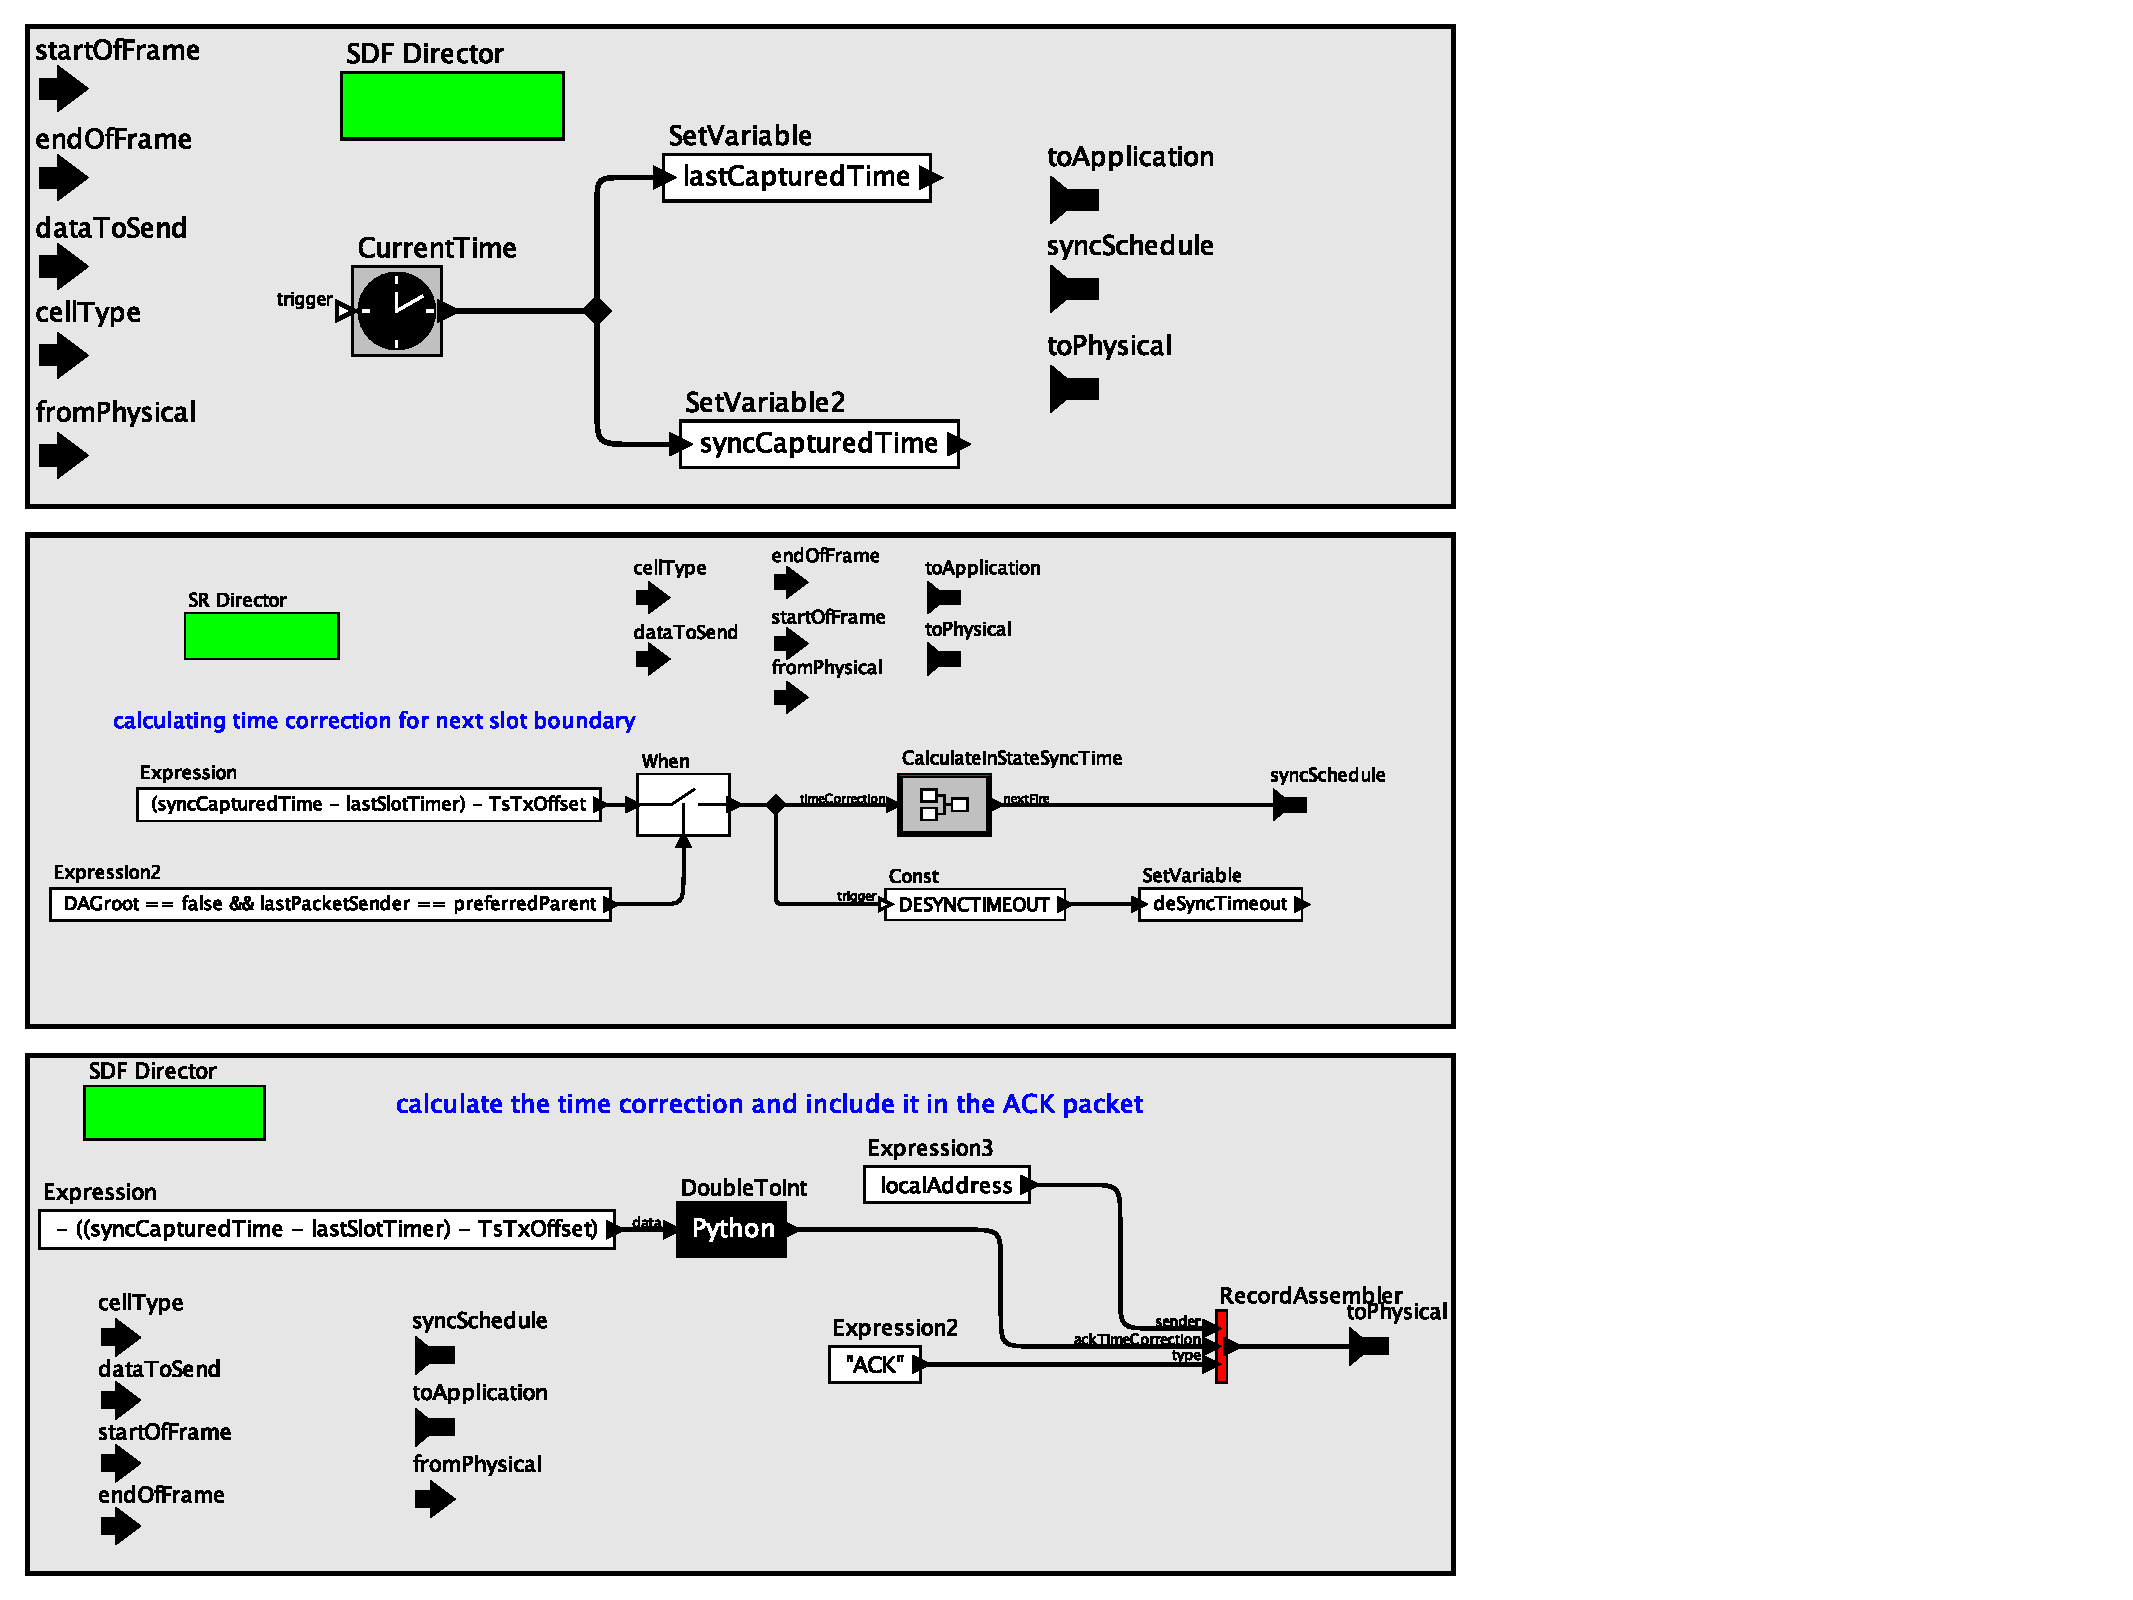
\includegraphics[width=0.9\columnwidth]{figures/PaperReSynchronization}
\caption{Modelling the the resynchronization.}
\label{fig:timeCorrection}
\end{figure}



%%% Local Variables: 
%%% mode: latex
%%% TeX-master: "ee219d"
%%% End: 
